\documentclass[11pt, 12pt, twoside, onecolumn]{book}

\usepackage[english]{babel} 			%language selection
\selectlanguage{english}

\usepackage{amsmath}    				% Include the AMS Mathematics package.
\usepackage{hyperref}      				   % Include the hyper reference package.
\usepackage{draftwatermark}			 % Be able to add watermarks.

% Add a DRAFT watermark to the document.
\SetWatermarkLightness{0.85}
\SetWatermarkScale{1.5}
\SetWatermarkText{DRAFT}

% Include packages for dealing with fonts.
\usepackage[T1]{fontenc}
\usepackage{cmbright}

% Include packages for dealing with page layout.
\usepackage{geometry}
\usepackage{pdflscape}
\usepackage{fancyhdr}

% Include packages for dealing with graphics.
\usepackage{placeins}
\usepackage{graphicx}     					% Include the graphics package.
\usepackage{caption}
\usepackage{subcaption}
\usepackage{floatflt}

% Setup the format of hyperlinks.
\hypersetup{colorlinks, citecolor=black, filecolor=black, 
			linkcolor=black, urlcolor=blue, bookmarksopen=true, 
			pdftex}

% Set the page-styles.
\pdfpagewidth 8.5in
\pdfpageheight 11in
%\pagestyle{plain}
%\pagenumbering{arabic}
\setlength{\headheight}{15.2pt}

\pagestyle{fancy}
\fancyhead{}								% clear all header fields
\fancyhead[RO,LE]{\bfseries Process Guideline for Using the RelKit Application to Implement LRM}
\fancyfoot{}								% clear all footer fields
\fancyfoot[C]{\thepage}

% Unique commands used in this document.
\newcommand{\code}[1]{\textrm{\textit{#1}}}
\renewcommand{\headrulewidth}{0.6pt}
\renewcommand{\footrulewidth}{0.4pt}

\begin{document}

% Set up font information for the entire document.
\fontencoding{T1}
\fontfamily{cmbright}
\fontseries{l}
\fontshape{n}
\selectfont
\normalfont

\captionsetup{labelfont=bf}

\begin{titlepage}
\centering
{\linespread{1.3} \Huge \textbf{Using the RelKit Application to Implement the LRM Process}} \\
\vspace{5in}
{\linespread{1.3} \large \textbf{Andrew Rowland}} \\
{\linespread{1.3} \large \textbf{ReliaQual Associates, LLC}}
\end{titlepage}

\tableofcontents
\newpage

\chapter{Overview}
\FloatBarrier
\noindent The RelKit application is a software toolkit that can be used to help manage the Lifecycle Reliability Management (LRM) process.  RelKit can be used to assist in the following LRM tasks:

	\begin{itemize}
		\item Warranty Analysis
		\item Reliability Risk Analysis
		\item Reliability Capability Analysis
		\item Reliability Risk Indexing
		\item Reliability Growth Planning
		\item Reliability Growth Tracking
	\end{itemize}

\section{RelKit Software}
\FloatBarrier
\noindent This section provides a brief description of the RelKit software.

\section{Definitions}\label{def}
\FloatBarrier
\noindent The following is a list of abbreviations and terms that are used throughout this manual.

	\begin{enumerate}
		\item \textbf{LRM} - Lifecycle Reliability Management
		\item \textbf{RelKit Program} - this is a RelKit database.
	\end{enumerate}
	
\chapter{Creating a New RelKit Program}
\FloatBarrier
\noindent To use the RelKit software for managing LRM projects, you will need to create a RelKit Program.  After creating a new RelKit Program, you will need to populate it with system hardware and warranty claim information.  Creating a new RelKit Program for a LRM project requires the following steps, at minimum:

	\begin{enumerate}
		\item Select 'New Program' from either the toolbar or the \textit{File} menu.
		\item Either:
		\begin{enumerate}
			\item Manually create the system hardware structure.
			\item Import the system hardware structure from an external file.
		\end{enumerate}
		\item Either:
		\begin{enumerate}
			\item Manually enter all of the warranty claim information.
			\item Import all of the warranty claim information from an external file.
		\end{enumerate}
	\end{enumerate}

\noindent Figure \ref{fig:new_project_hardware} shows RelKit with the newly created RelKit Program open and selected to the Hardware tree tab.  With a new project, there is only one line in the Hardware tree for the top-level assembly, or system.  At this point it is necessary to create the remainder of the product structure.  This can be done either by manually creating all of the remaining structure or by importing the information from an external file. \\

\begin{landscape}
		\begin{figure}[htbp]
			\centering
			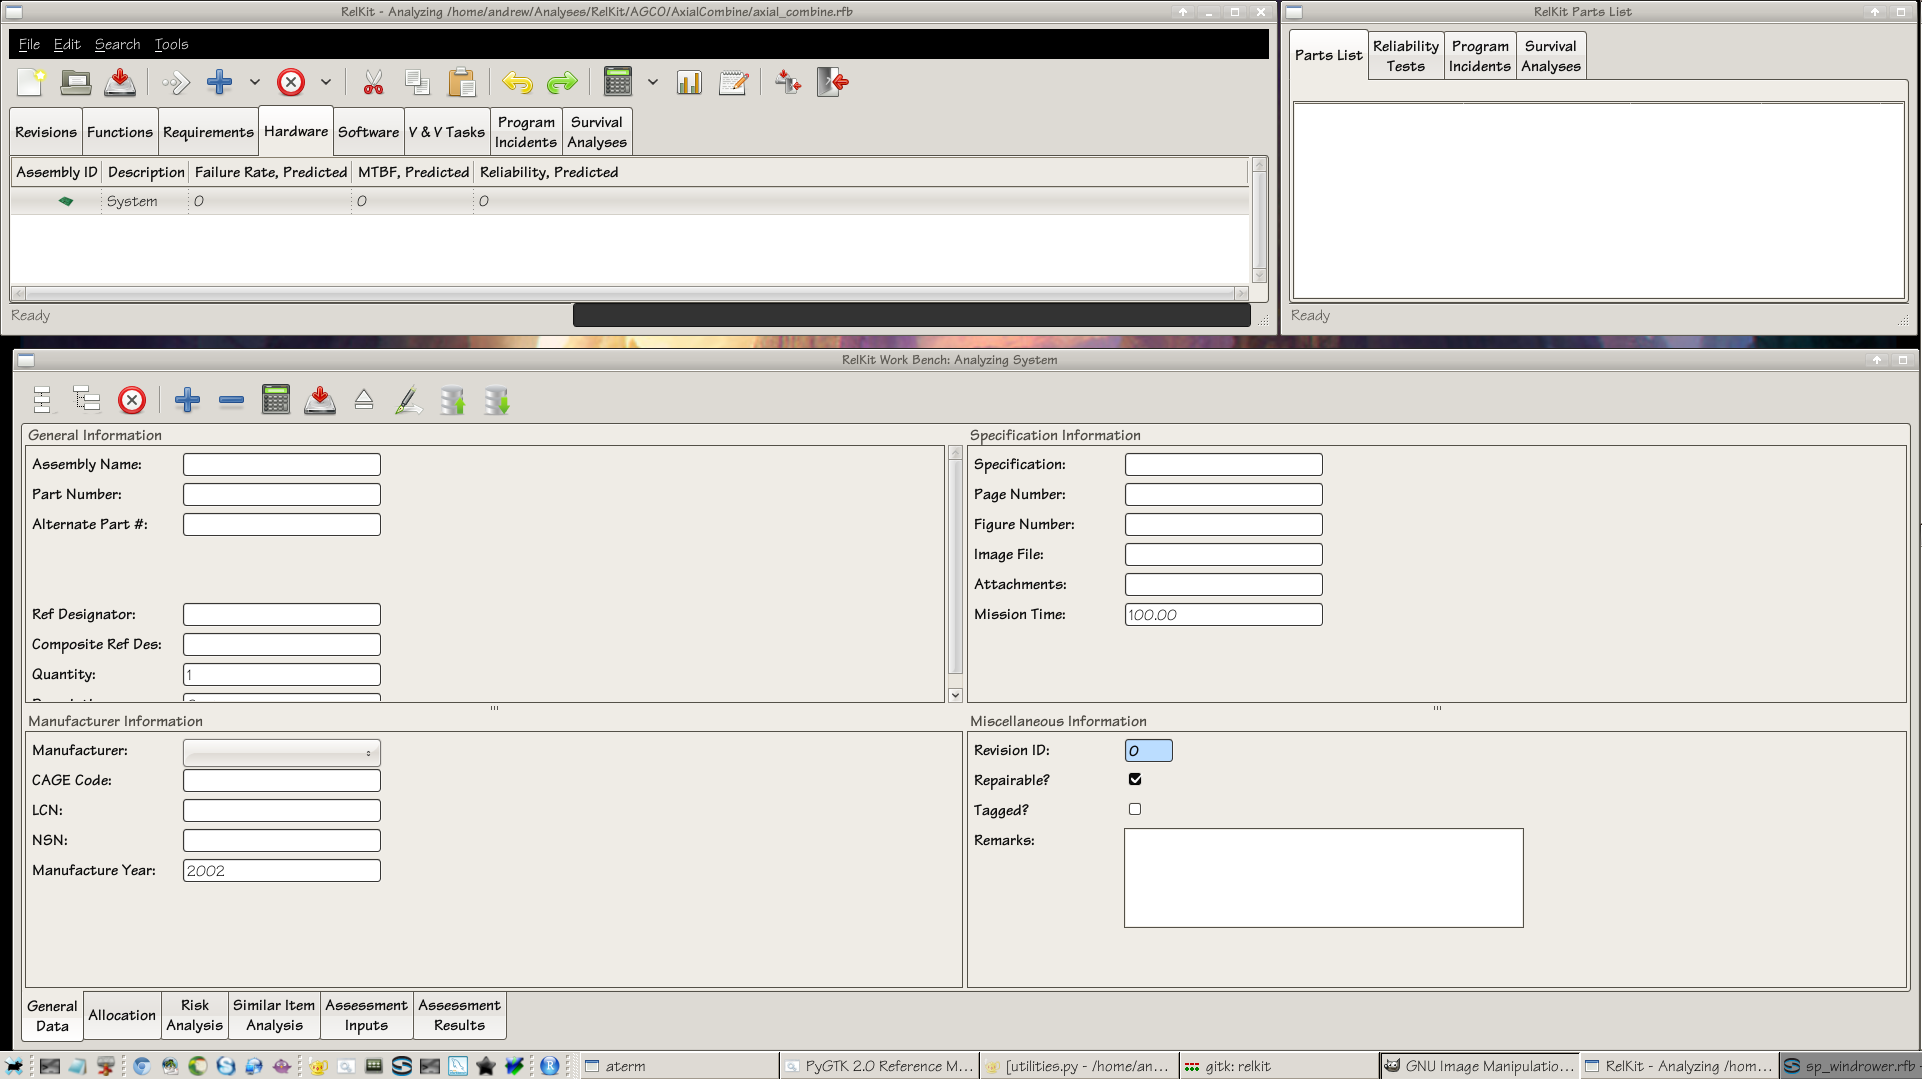
\includegraphics[width=18cm]{./figures/new_project_hardware}
			\caption{\textbf{New RelKit Project}}
			\label{fig:new_project_hardware}
		\end{figure}
\end{landscape}

\section{Manually Building the Hardware Structure}

\noindent To manually build the hardware structure, you will use the "Add Sibling Assembly" (Figure \ref{fig:add_sibling_assembly}) and "Add Child Assembly" (Figure \ref{fig:add_child_assembly}) tool buttons found on the RelKit Workbench tool bar.  All new assemblies are added with reference to the currently selected hardware item.  Thus, with a new RelKit Program, only the top-level assembly will be available. \\

\begin{figure}[htb]
	\begin{minipage}{0.5\textwidth}
		\centering
		\subcaptionbox{\label{fig:add_sibling_assembly}}{
\includegraphics[width=32pt]{./figures/insert_sibling}} \quad \quad \quad
		\subcaptionbox{\label{fig:add_child_assembly}}{
\includegraphics[width=32pt]{./figures/insert_child}}
	\end{minipage}\hfill
	\caption{\textbf{Add Hardware Tool Buttons}}
	\label{fig:add_hardware}
\end{figure}

\noindent Selecting to add a sibling assembly will result in the dialog in Figure \ref{fig:add_sibling_dialog} being displayed.  In this dialog, enter the number of sibling assemblies you wish to add and press the 'OK' button.  This will add the specified number of assemblies at the same indenture level as the selected hardware item.  Note that RelKit will not allow you to add a sibling assembly to the top-level hardware item.  Adding child assemblies occurs in a similar manner. \\

\noindent Once the hardware structure is constructed through the use of the "Add Sibling Assembly" and "Add Child Assembly" tool buttons, additional information such as the description or the name of each assembly must be manually entered.  This is accomplished by first selecting the hardware item you wish to edit.  With the hardware item selected, information related to the item can be added or edited in the RelKit Workbench window. \\

\section{Importing the Hardware Structure}

\noindent Figure \ref{fig:import_hardware} shows the assistant used to import the hardware structure.  Figure \ref{fig:select_file} shows the dialog used to select the source file.  Matching the source file columns to the appropriate database fields is done with the dialog shown in Figure \ref{fig:match_columns}.  A source column may be assigned to multiple database fields.  It is recommended that the Description and Name fields in the database be mapped to the same source file column unless the source file has a unique column for each. \\

\noindent Finally, Figure \ref{fig:new_project_hardware_after_import} shows the Hardware Tree after the import.  Note the default name of the top-level assembly has been updated.  All fields for existing assemblies will be updated with new information if available.  Also, we can two of the assemblies subordinate to the top-level assembly. \\

\begin{figure}[htbp]
	\centering
	\begin{subfigure}[b]{0.6\textwidth}
		\centering
        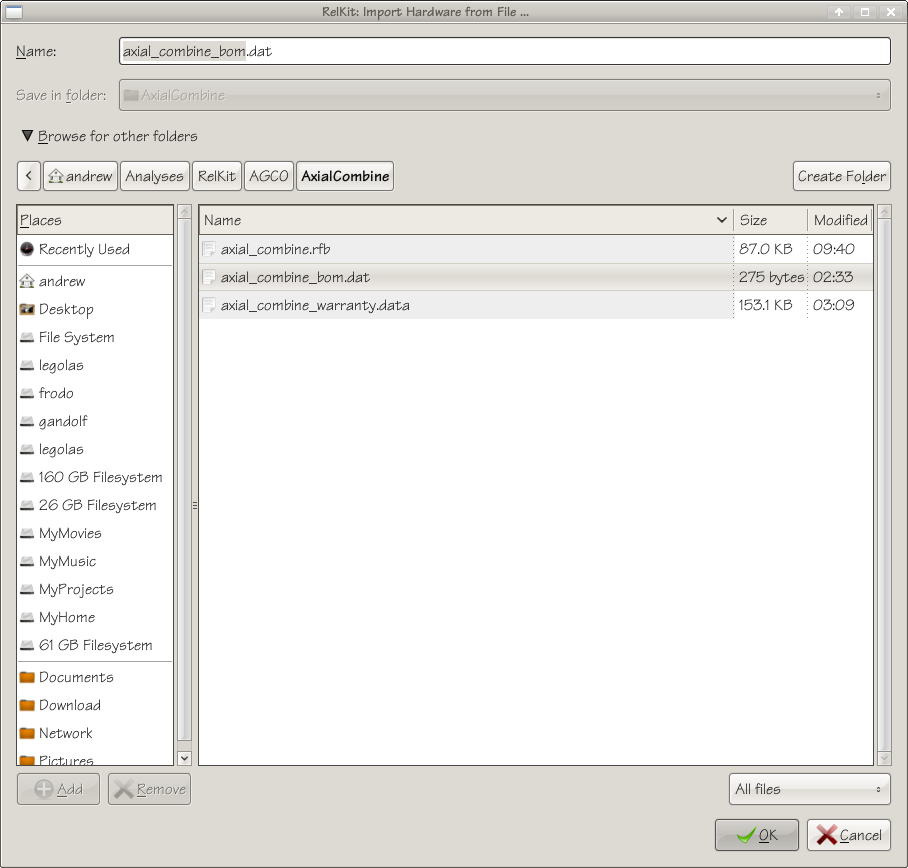
\includegraphics[width=\textwidth]{./figures/new_project_import_bom_1}
        \caption{\textbf{Select Source File}}
        \label{fig:select_file}
	\end{subfigure}
	\\
   	\begin{subfigure}[b]{0.6\textwidth}
   		\centering
        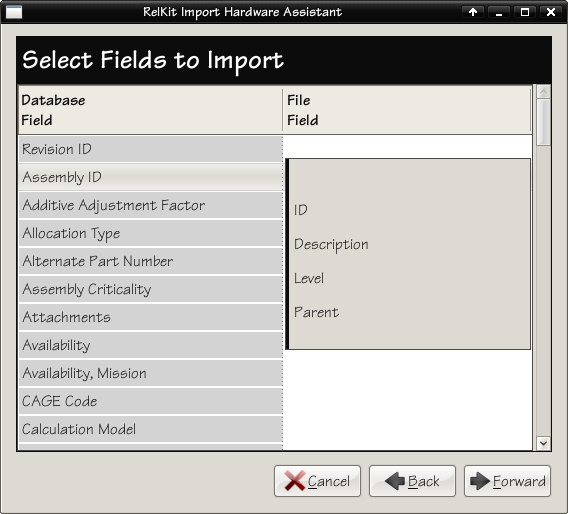
\includegraphics[width=\textwidth]{./figures/new_project_import_bom_2}
        \caption{\textbf{Assign Source Columns to Database Fields}}
        \label{fig:match_columns}
	\end{subfigure}
	\caption{\textbf{Importing Hardware Structure to RelKit}}
	\label{fig:import_hardware}
\end{figure}
	
\begin{landscape}
	\begin{figure}[htbp]
		\centering
		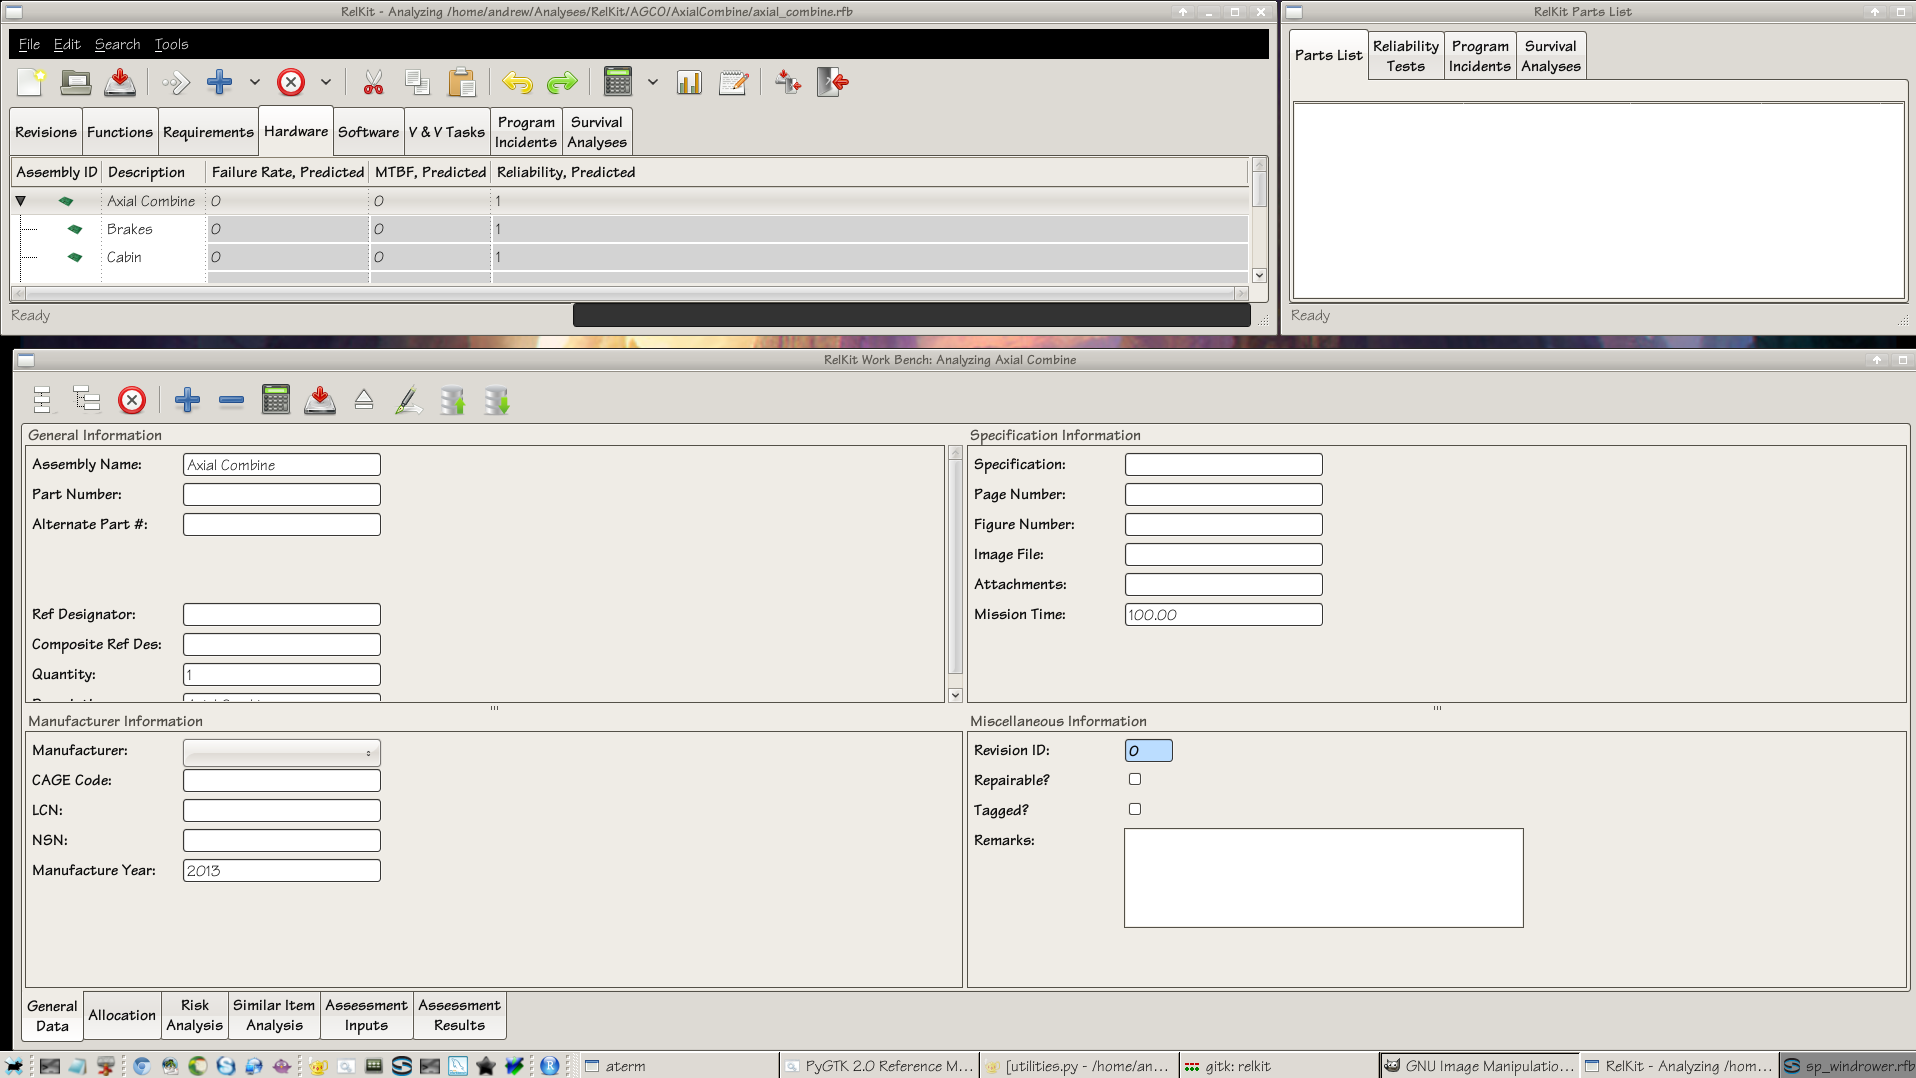
\includegraphics[width=18cm]{./figures/new_project_import_bom_3}
		\caption{\textbf{Hardware Tree After Importing}}
		\label{fig:new_project_hardware_after_import}
	\end{figure}
\end{landscape}

	
\end{document}